\documentclass[final,12pt]{article}    
%%%%%%%%%%%%%%%%%%%%%%%%%%%%%%%%%%%%%%%%%%%%%%%%%%%%%%%%%%%%%
%
%  include packages
%
\usepackage{times}
\usepackage{ifthen}
\usepackage{graphics}
\usepackage{color}
\usepackage{shadow}
%%%%%%%%%%%%%%%%%%%%%%%%%%%%%%%%%%%%%%%%%%%%%%%%%%%%%%%%%%%%%
%
%  if private=false certain descriptions are excluded using
%  the \ifthenelse expression
%
\newboolean{private}\setboolean{private}{true}
\newboolean{qmmm}\setboolean{qmmm}{true}
%%%%%%%%%%%%%%%%%%%%%%%%%%%%%%%%%%%%%%%%%%%%%%%%%%%%%%%%%%%%%
%
%  define commands
%
\newcommand{\block}[1]{\subsubsection[#1]{\shabox{\bf #1}}}
%
\newcommand{\brules}[1]{
\makebox[1in][l]{Rules:}\parbox[t]{110mm}{#1}\hfill\break\hfill}
%
\newcommand{\bdescr}[1]{
\makebox[1in][l]{Description:}\parbox[t]{110mm}{#1}\hfill\break}
%
%\newcommand{\key}[1]{\hfill\break
%\makebox[1in][l]{Keyword:}\parbox[t]{110mm}{{\bf #1}}\hfill\break}
%
\newcommand{\key}[1]{\hfill\break \makebox[1.5in][l]{\bf #1}\hfill\break}
%
%\newcommand{\vdescr}[1]{
%\makebox[1in][l]{}\parbox[t]{110mm}{#1}\hfill\break}
%
\newcommand{\vdescr}[1]{\makebox[1in][l]{}\parbox[t]{110mm}{#1}\hfill\break}
%
\newcommand{\vformat}[1]{
\makebox[1in][l]{}\parbox[t]{110mm}{\makebox[1in][l]{Type:}\parbox[t]{2.7in}{#1}}
\hfill\break}
%
\newcommand{\vrules}[1]{
\makebox[1in][l]{}\parbox[t]{110mm}{\makebox[1in][l]{Rules:}\parbox[t]{2.7in}{#1}}
\hfill\break}
%
\newcommand{\vdefault}[1]{
\makebox[1in][l]{}\parbox[t]{110mm}
{\makebox[1in][l]{Default:}\parbox[t]{2.7in}{#1}}
\hfill\break}
%
\newcommand{\mbax}[1]{#1}
%============================================================
%%%%%%%%%%%%%%%%%%%%%%%%%%%%%%%%%%%%%%%%%%%%%%%%%%%%%%%%%%%%%
%
% prepare titlepage
%
\title{{\bfseries\Huge 
    \hrulefill\\
    \hrulefill Changes of the \hrulefill\\
    \hrulefill \hrulefill Projector Augmented Wave \hrulefill\\
    \hrulefill Method \hrulefill\\}
    \medskip{\LARGE Version 2.0}\\
%\thanks{Peter~E.~Bl\"ochl, Clausthal University of Technology \date}\\   
%\resizebox{!}{9.0cm}{\includegraphics[10mm,15mm][90mm,110mm]{big.eps}}
\resizebox{!}{9.0cm}{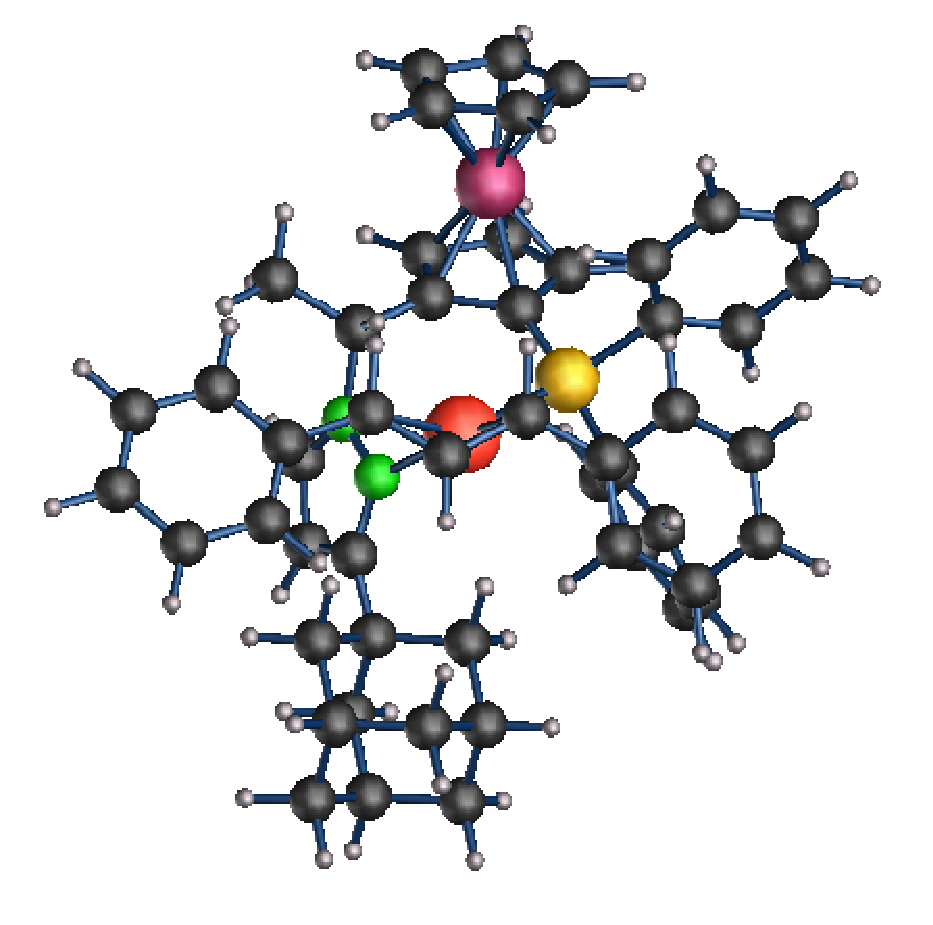
\includegraphics{big.eps}}
}
\date{\hrulefill\\Peter~E.~Bl\"ochl, Clausthal University of Technology\\(\today)}

\begin{document}          
\maketitle   
%
\noindent            
\setcounter{page}{1}
\footnote{The title picture shows the a chiral Pd complex with P,N ligands,
  a highly enantio-selective catalyst for allylic amination \cite{Pdcat}.}
\newpage
\tableofcontents
%==========================================================================
\newpage
\setcounter{page}{1}
%==========================================================================
\section{Changes}
%==========================================================================
\begin{itemize}
\item Apr. 28,2001; P.E. Bloechl; The selection of k-points has been
changed.  In \texttt{!Structure!Kpoint} an equispaced grid is selected
with either \texttt{R} or \texttt{DIV}. The Gamma point is obtained
when \texttt{!Structure!Kpoint} is not selected or with \texttt{DIV=0 0
0}. When \texttt{DIV} is selected also individual k-points can be
chosen.
\end{itemize}
%==========================================================================
\section{ToDo}
%==========================================================================
\begin{itemize}
\item in paw\_augmentation there is still a ``severe warning'' for
calculating the background charge. 
\item Offcenter wave function mass for spinor wave functions and
offdiagonal mass for occupations with spin-polarisation.
\item For the cell dynamics we need the retoring force for the plane
wave coinvergence.
\end{itemize}
%==========================================================================
\section{Done}
%==========================================================================
\begin{itemize}
\item after removing the source blas and lapack routines the linker
could not resolve the following references. Solution do not use the
lapack from atlas but the source version.

\begin{verbatim}
/usr/absoft/lib/libfio.a(lowlevel.o): In function `_temp_file':
lowlevel.o(.text+0x10): the use of `tempnam' is dangerous, better use `mkstemp'
/home/blo/Tree/PAW//Objects/dbg/paw_library.o: In function `passf5_':
paw_library_d.f90:407: undefined reference to `dgetri_'
paw_library_d.f90:468: undefined reference to `dspev_'
paw_library_d.f90:547: undefined reference to `zhpev_'
paw_library_d.f90:1294: undefined reference to `dgelss_'
/home/blo/Tree/Libraries/Packages/ATLAS//lib/Linux_ATHLON//liblapack.a(ATL_dgetrfC.o): In function `ATL_dgetrfC':
ATL_dgetrfC.o(.text+0xf1): undefined reference to `cblas_dtrsm'
ATL_dgetrfC.o(.text+0x131): undefined reference to `cblas_dgemm'
ATL_dgetrfC.o(.text+0x1b9): undefined reference to `cblas_idamax'
ATL_dgetrfC.o(.text+0x201): undefined reference to `cblas_dscal'
/home/blo/Tree/Libraries/Packages/ATLAS//lib/Linux_ATHLON//liblapack.a(ATL_dgetrfR.o): In function `ATL_dgetrfR':
ATL_dgetrfR.o(.text+0xf2): undefined reference to `cblas_dtrsm'
ATL_dgetrfR.o(.text+0x130): undefined reference to `cblas_dgemm'
ATL_dgetrfR.o(.text+0x1b5): undefined reference to `cblas_idamax'
ATL_dgetrfR.o(.text+0x1f9): undefined reference to `cblas_dscal'        
\end{verbatim}
\end{itemize}

\end{document}
\bye
